\documentclass[conference]{IEEEtran}
\usepackage[T1]{fontenc}
\usepackage{cite}
\usepackage{amsmath,amssymb}
\usepackage{graphicx}
\usepackage{booktabs}
\usepackage{placeins}
\usepackage{url}
\usepackage[hidelinks]{hyperref}
\graphicspath{{figures/}}
\newcommand{\degC}{\ensuremath{^\circ\mathrm{C}}}
\hyphenation{Sales-force fore-cast-ing}
\begin{document}
\title{Benchmarking Multi-Step Sensor Forecasting for Threshold-Based Predictive Maintenance: An Integrated IoT-to-Enterprise Framework}
\author{\IEEEauthorblockN{Wahaj Raza, Huzaifa Naseer Khan, Farrukh Niaz, and Muzammil Rizvi}
\IEEEauthorblockA{Department of Computer System Engineering\\
NED University of Engineering \& Technology, Karachi, Pakistan\\
\{wahajraza6, huzaifanaseerkhan02, osamaniaz466, muzammilrizvi977\}@gmail.com}}
\maketitle

\begin{abstract}
Sensor forecasting can support maintenance planning when forecasts are connected to monitoring, threshold alerts, and service workflows. This paper presents an integrated IoT-to-enterprise prototype and a comparative evaluation of 24-hour multi-step sensor forecasting. The prototype combines ESP32-S3 acquisition, GPS, DS18B20 temperature sensing, BLE tyre-pressure monitoring, HTTP telemetry, and the Swift platform, with Salesforce alert ingestion and status feedback. Its documented maintenance workflow uses Cases and Flow; the available repository evidence supports integration components rather than a measured operational deployment. A corrected benchmark evaluates persistence, seasonal naive, Random Forest, and a bidirectional long short-term memory (Bi-LSTM) network on three synthetic sensor datasets, using seven days of historical target values and chronological partitions with disjoint target periods. We add five-seed Bi-LSTM robustness, an LSTM/Bi-LSTM architecture comparison, causal feature ablation, proxy threshold-event scoring, moving-block bootstrap intervals, and external sensor-forecasting evaluation on the NASA C-MAPSS FD001 simulator benchmark. Random Forest achieves the lowest mean absolute error for engine temperature (1.708\degC) and tyre temperature (2.897\degC), while persistence performs best for tyre pressure (0.558 PSI). The C-MAPSS and feature experiments use a separately recorded TensorFlow/scikit-learn environment, which is retained as a reproducibility limitation. The evaluation does not establish failure prediction, real-fleet deployment, or maintenance-outcome benefits.
\end{abstract}
\begin{IEEEkeywords}
Internet of Things, multi-step forecasting, predictive maintenance, Random Forest, Bi-LSTM, enterprise maintenance workflow.
\end{IEEEkeywords}

\section{Introduction}
Vehicle maintenance decisions require both visibility into asset condition and a process for acting on that information. A dashboard can display abnormal readings, but an actionable maintenance workflow also needs an asset identifier, an alert description, an assigned service task, and feedback on its status. Predictive-maintenance architectures therefore combine data acquisition, analysis, and decision processes; forecasting quality is only one part of this chain~\cite{zhu2024}.

The intended application of AutoSense is vehicle monitoring, including the aviation ground-support context that motivated the prototype. The available evidence does not establish deployment in an operational aviation fleet. We study the narrower task of forecasting engine temperature, tyre pressure, and tyre temperature over the next 24 hours, with forecasts intended to inform threshold-based maintenance alerts. Predicting a threshold excursion is distinct from predicting a component failure: no failure-time, remaining-useful-life, or maintenance-outcome labels are available here.

The forecasting study compares models under a shared protocol instead of assuming that a recurrent neural network is the strongest choice. Straightforward forecasting methods provide essential reference points~\cite{hyndman2021}. We separate two kinds of evidence: repository artifacts describing a telemetry-to-service prototype, and numerical results from a reproducible synthetic-data benchmark. This separation prevents interface demonstrations from being interpreted as forecast validation.

The contributions are: (1) an IoT-to-maintenance workflow prototype connecting telemetry, monitoring, forecasting interfaces, alerts, and enterprise status feedback; (2) a standardized 24-hour forecasting benchmark for three sensor variables with consistent information access and disjoint target periods; (3) robustness, architecture, feature, threshold-event, and dependence-aware uncertainty analyses; (4) a C-MAPSS FD001 external simulated-benchmark sensor-forecasting study with engine-level separation; and (5) an evidence-bounded account of Salesforce maintenance integration. The contribution is comparative evaluation and system integration, rather than a new forecasting algorithm or a claim of Bi-LSTM superiority.

\section{Related Work}
\subsection{Predictive Maintenance and Fleet Monitoring}
Condition-based maintenance is commonly framed as data acquisition, data
processing, and maintenance decision-making~\cite{jardine2006}. Reviews of
machine-learning predictive maintenance likewise emphasize that performance is
task- and data-dependent rather than a property of a model family in
isolation~\cite{carvalho2019,zhu2024}. This motivates separating the present
forecasting metrics from the unmeasured downstream maintenance decision. Fleet
monitoring is the application context here; labelled maintenance outcomes would
be required to evaluate breakdown avoidance, cost, or downtime.

\subsection{IoT Maintenance Architectures}
Cloud-enhanced maintenance architectures connect acquisition and analytical components~\cite{zhu2024}. In our implementation, an ESP32-S3 provides the acquisition and wireless communication platform, while the DS18B20 provides a digital temperature interface~\cite{esp32,ds18b20}. These component references establish device capabilities, not automotive qualification, sensing accuracy in the installed configuration, or end-to-end reliability. The prototype's concrete evidence consists of firmware, a circuit schematic, interface captures, and integration code.

\subsection{Sensor Time-Series Forecasting}
Naive and seasonal naive methods establish useful forecasting benchmarks~\cite{hyndman2021}. Random Forest combines randomized tree predictors~\cite{breiman2001}, providing a nonlinear model of lagged target values without recurrent state. LSTM introduces gated recurrent memory~\cite{hochreiter1997}, while bidirectional recurrent processing encodes a sequence in both temporal directions~\cite{schuster1997}. In forecasting, both directions may process the observed input window without accessing future targets. These methodological foundations justify the comparison; they do not imply superior predictive-maintenance performance for a particular architecture.

\subsection{External Simulated Degradation Benchmarks}
NASA's C-MAPSS repository provides simulator-generated run-to-failure turbofan
trajectories under controlled operating and fault settings~\cite{saxena2008}.
Many C-MAPSS studies target remaining useful life (RUL). That task is deliberately different from ours: we
forecast four observed sensors ten cycles ahead from complete FD001 training
trajectories, and use normalized life only after prediction to stratify error.
Thus no C-MAPSS RUL score or physical-flight-telemetry claim is made.

\begin{table*}[t]
\caption{Compact, verifiable positioning of this study. ``Decision/workflow''
means an evaluated downstream decision, not merely an architecture diagram.}
\label{tab:related-work}
\centering\small
\setlength{\tabcolsep}{2pt}
\begin{tabular}{p{1.65cm}p{2.7cm}p{2.7cm}p{3.65cm}p{3.55cm}}
\toprule
Study & Setting and provenance & Forecasting or maintenance scope & Methods and metrics & Decision/workflow evidence \\
\midrule
Jardine \emph{et al.}~\cite{jardine2006} & Mechanical systems; review literature & Condition monitoring, diagnostics, and prognostics & Review of models and algorithms; no single metric set & Reviews maintenance decision support \\
Carvalho \emph{et al.}~\cite{carvalho2019} & Industrial PdM; systematic-review literature & Machine-learning predictive maintenance & Review of ML methods; study-dependent metrics & No common workflow experiment \\
Saxena and Goebel~\cite{saxena2008} & Simulated turbofan engines; NASA C-MAPSS & Run-to-failure benchmark resource & Dataset resource, not a model study & None \\
This work & Synthetic AutoSense; simulated C-MAPSS FD001 & Multi-step sensor forecasting; proxy threshold events & Naive, RF, LSTM, Bi-LSTM; MAE, RMSE, $R^2$, event metrics & Prototype artifacts only; no evaluated maintenance outcome \\
\bottomrule
\end{tabular}

\end{table*}

\subsection{Enterprise Maintenance Workflow Integration}
Salesforce Flow supports record-triggered criteria and record-creation actions~\cite{salesforceflow}. Such mechanisms can translate an alert into a service workflow. Product documentation establishes that capability, whereas deployment-specific validation requires configuration exports and execution evidence. We describe the available alert-ingestion and vehicle-status code separately from the Case/Flow linkage documented in the original project narrative.

\section{System Architecture}
Fig.~\ref{fig:architecture} summarizes the logical integration. The on-vehicle sensor layer combines GPS location, DS18B20 temperature sensing, and BLE TPMS pressure and temperature readings. The ESP32-S3 firmware contains GPS parsing, OneWire temperature acquisition, BLE advertisement parsing, JSON payload construction, and HTTP POST transmission. The stored PCB schematic documents the hardware design. Neither its existence nor the firmware demonstrates environmental qualification or calibrated engine-condition measurement.

\begin{figure*}[t]
\centering
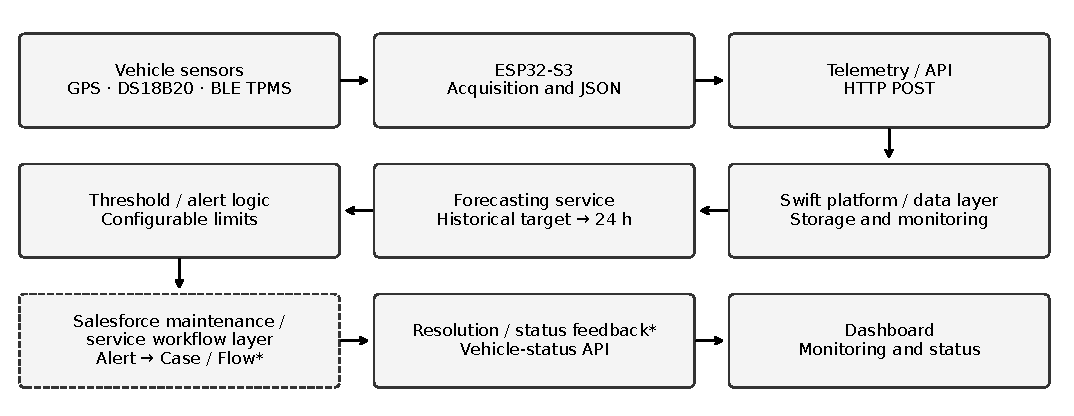
\includegraphics[width=\textwidth]{system_architecture.pdf}
\caption{Logical IoT-to-enterprise architecture. Arrows represent intended information flow rather than measured transaction traces. *Case/Flow automation and its resolution linkage are documented in the original project narrative; exported Flow configuration and execution logs are unavailable. Alert ingestion and vehicle-status feedback have repository code.}
\label{fig:architecture}
\end{figure*}

The Swift platform is the telemetry and visualization layer. Repository scripts fetch vehicle and sensor records, construct forecasting inputs, and format predictions for platform ingestion. Those integration scripts reference legacy neural models. The corrected offline benchmark reported here is a separate analysis; it has not been substituted into the deployed prototype or validated through a live forecast endpoint. In particular, the benchmark's time alignment must not be inferred from legacy dashboard timestamps.

Threshold logic connects readings or forecast excursions to alerts. For a target with configured acceptable bounds $[a,b]$, a possible forecast-alert rule is
\begin{equation}
A_t=\mathbb{1}\{\exists h\in\{1,\ldots,H\}:\hat y_{t+h|t}<a\ \text{or}\ \hat y_{t+h|t}>b\}.
\label{eq:alert}
\end{equation}
Equation~\ref{eq:alert} states the intended threshold semantics. Bounds must
be appropriate to the sensor placement and asset; a threshold displayed in a
screenshot is a configured prototype value, not a validated safety limit. We
do report offline precision, recall, F1, false-positive rate, and an
origin-level lead-time convention for training-derived proxy excursion labels.
Those labels are neither failures nor certified engineering alarms, and no
maintenance effectiveness is estimated.

Salesforce is the maintenance/service workflow layer. The available Apex code imports alerts into a custom Vehicle Alert object, checks existing alert identifiers before inserting records, and sends vehicle-status updates back to Swift through an asynchronous callout. The original project describes Cases and Flow for maintenance-task creation and resolution feedback. Because those Flow definitions are not exported in the repository, that part of the diagram remains a documented integration design, rather than independently reproduced Case automation.

\section{Forecasting Methodology}
\subsection{Synthetic Data and Time Validation}
All three benchmark series are synthetic. The repository's generators reproduce their timestamps exactly and their target values to floating-point precision (maximum absolute discrepancy below $1.5\times10^{-14}$). Thus, the presence of physical sensor hardware does not establish sensor-collected provenance for these datasets. Each file covers 2024 from January 1 through December 31 at 00:00 in its recorded clock; the final day is not fully sampled. No timezone is inferred.

The corrected protocol rejects missing timestamps, duplicate or unsorted timestamps, non-finite target values, and irregular sampling. No implicit sorting, interpolation, or resampling is performed. Engine temperature is hourly; tyre pressure and tyre temperature are sampled every three hours. Table~\ref{tab:protocol} records the resulting window counts. A seven-day input contains 168 hourly samples or 56 three-hour samples. A 24-hour output contains 24 hourly steps or eight three-hour steps. Horizon labels denote time after the last observed input sample.

\begin{table*}[t]
\caption{Dataset and protocol summary. Train, validation, and test columns count complete forecast windows; every dataset is synthetic.}
\label{tab:protocol}
\centering\small
\setlength{\tabcolsep}{4pt}
\begin{tabular}{llrrrrrrrl}
\toprule
Target & Type & Rows & Step (h) & Lookback (h) & Horizon (h) & Train & Val. & Test & Unit \\
\midrule
Engine temperature & Synthetic & 8761 & 1 & 168 & 24 & 5765 & 1029 & 1730 & $^\circ$C \\
Tyre pressure & Synthetic & 2921 & 3 & 168 & 24 & 1922 & 344 & 578 & PSI \\
Tyre temperature & Synthetic & 2921 & 3 & 168 & 24 & 1922 & 344 & 578 & $^\circ$C \\
\bottomrule
\end{tabular}

\end{table*}

\subsection{Chronological Partitioning}
For a series of $N$ raw rows, the test region starts at $b_t=\lfloor0.8N\rfloor$ and validation starts at $b_v=\lfloor0.85b_t\rfloor$. These boundaries allocate approximately 68\% to fitting, 12\% to validation, and 20\% to testing. A window is assigned only if its entire target sequence lies inside one region. Windows with targets crossing either boundary are excluded. Consequently, training, validation, and test target timestamps do not overlap.

Inputs may include observations from an earlier region, since they are historical information available at that forecast origin. Test origins advance one sample at a time, and later test inputs may contain previously observed test-period values. This is rolling-origin evaluation with fixed trained parameters, not a single open-loop forecast from the start of the holdout. There is no refitting on validation or test observations. Within each partition, overlapping target windows produce dependent errors.

All four models share test origins and targets. Both learned models use only the historical target sequence, with no GPS, calendar, cross-sensor, or engineered covariates. The Random Forest uses the sequence as a lag vector; the network uses it as a univariate sequence. Min--max scaling for the network is fitted only on the fitting-region raw values. Forecasts are inverse-transformed before scoring. This protocol also avoids the earlier baseline utility's target overlap caused by splitting already-constructed windows. Legacy notebook results with different features or splits are not mixed into the comparison.

\subsection{Forecasting Models}
Persistence repeats the latest observed target across the horizon. Seasonal naive repeats the immediately preceding 24-hour pattern; the seasonal period is therefore 24 samples for engine temperature and eight for the tyre targets. Both baselines require no parameter fitting.

Random Forest is a direct multi-output regressor with 300 trees, maximum depth 16, minimum leaf size two, and random state 42. It predicts the whole output vector from the lag vector and uses the same fitting windows as the neural model. The unchanged implementation uses scikit-learn defaults for other parameters.

The evaluated network, labelled Bi-LSTM, contains a bidirectional LSTM with 128 units per direction and sequence output, batch normalization, dropout 0.2, a second bidirectional LSTM with 64 units per direction and sequence output, batch normalization, dropout 0.3, a unidirectional LSTM with 32 units, a dense ReLU layer with 64 units, dropout 0.2, and a linear output layer of size $H$. Bidirectionality is confined to historical inputs. The architecture is a mixed recurrent stack, not a claim that every recurrent layer is bidirectional.

\subsection{Evaluation Metrics}
Let $M$ be the number of test origins, $H$ the number of forecast steps, and $e_{ih}=y_{ih}-\hat y_{ih}$. Metrics are pooled over all origin--horizon pairs:
\begin{align}
\mathrm{MAE}&=\frac{1}{MH}\sum_{i=1}^{M}\sum_{h=1}^{H}|e_{ih}|,\\
\mathrm{RMSE}&=\sqrt{\frac{1}{MH}\sum_{i=1}^{M}\sum_{h=1}^{H}e_{ih}^{2}},\\
R^2&=1-\frac{\sum_{i,h}e_{ih}^{2}}{\sum_{i,h}(y_{ih}-\bar y)^2},
\end{align}
where $\bar y$ is the pooled target mean. MAE and RMSE retain physical units; $R^2$ is dimensionless. Negative $R^2$ means worse squared error than the pooled-mean reference. Horizon-wise MAE averages across origins at each step. Pooling counts a timestamp more than once when predicted at different horizons; it is not a metric over unique timestamps.

\section{Experimental Setup}
The corrected single-seed benchmark, five-seed AutoSense Bi-LSTM study, and
architecture ablation record TensorFlow 2.18.0 and scikit-learn 1.9.0; the
five-seed study also records NumPy 2.0.2 and pandas 2.2.2. The C-MAPSS
forecasting and feature-ablation runs record TensorFlow 2.20.0 and
scikit-learn 1.6.1. The C-MAPSS stage analysis records TensorFlow 2.18.0 and
scikit-learn 1.9.0 but consumes forecasts from the 2.20.0/1.6.1 forecasting
run. This heterogeneous environment is a documented reproducibility
limitation, not a claim of uniform software execution.

Random seeds are fixed to 42 unless a phase explicitly uses the predeclared
five AutoSense seeds (11, 21, 42, 84, 168) or three C-MAPSS Bi-LSTM seeds
(11, 42, 84). Neural training uses Adam, mean squared error loss, batch size
64, no training-window shuffling, a 20-epoch cap, and validation-loss early
stopping with patience five and restored best weights. The feature study fixes
F0 (target history), F1 (target plus deterministic calendar), and F2 (target,
calendar, and causal lag/rolling features); it never uses centered windows.
No validation/test values select features, sensors, scalers, thresholds, or
hyperparameters.

The scientific source is the committed \texttt{research\_v2/results} and
\texttt{research\_v2/ieee\_results} artifact sets. Archive validation checks
source/data/protocol hashes, row counts, unique experiment keys, seed sets, and
recorded environments. For C-MAPSS FD001 it additionally checks the fixed
70/15/15 engine-level split, training-only selected sensors (9, 11, 14, and
12), 30-cycle lookback, 10-cycle horizon, and that all 44 prediction NPZs
contain only pre-registered test-engine IDs. Figure and table source hashes are
stored with the generated assets.

\section{Results and Discussion}
\subsection{Aggregate Comparison}
Table~\ref{tab:comparison} reports the complete corrected comparison, and Fig.~\ref{fig:mae} shows MAE with separate axes for the different target units. Random Forest achieves the lowest engine-temperature MAE (1.708\degC) and RMSE (2.262\degC), ahead of seasonal naive (2.623\degC\ MAE) and Bi-LSTM (6.199\degC\ MAE). Persistence has the largest engine MAE, 10.157\degC.

\begin{table*}[t]
\caption{Corrected test performance in physical units. Lower MAE/RMSE and higher $R^2$ are better. Bold marks the lowest MAE and RMSE within each target.}
\label{tab:comparison}
\centering\small
\begin{tabular}{llrrr}
\toprule
Target (unit) & Model & MAE & RMSE & $R^2$ \\
\midrule
Engine temperature ($^\circ$C) & Persistence & 10.157 & 12.474 & -0.799 \\
 & Seasonal naive & 2.623 & 3.449 & 0.862 \\
 & Random Forest & \textbf{1.708} & \textbf{2.262} & 0.941 \\
 & Bi-LSTM & 6.199 & 7.356 & 0.374 \\
\midrule
Tyre pressure (PSI) & Persistence & \textbf{0.558} & \textbf{0.979} & 0.804 \\
 & Seasonal naive & 0.781 & 1.241 & 0.686 \\
 & Random Forest & 0.736 & 1.003 & 0.795 \\
 & Bi-LSTM & 1.178 & 1.443 & 0.575 \\
\midrule
Tyre temperature ($^\circ$C) & Persistence & 5.786 & 7.105 & -0.840 \\
 & Seasonal naive & 3.897 & 4.964 & 0.102 \\
 & Random Forest & \textbf{2.897} & \textbf{3.680} & 0.507 \\
 & Bi-LSTM & 6.454 & 7.862 & -1.253 \\
\bottomrule
\end{tabular}

\end{table*}

\begin{figure*}[t]
\centering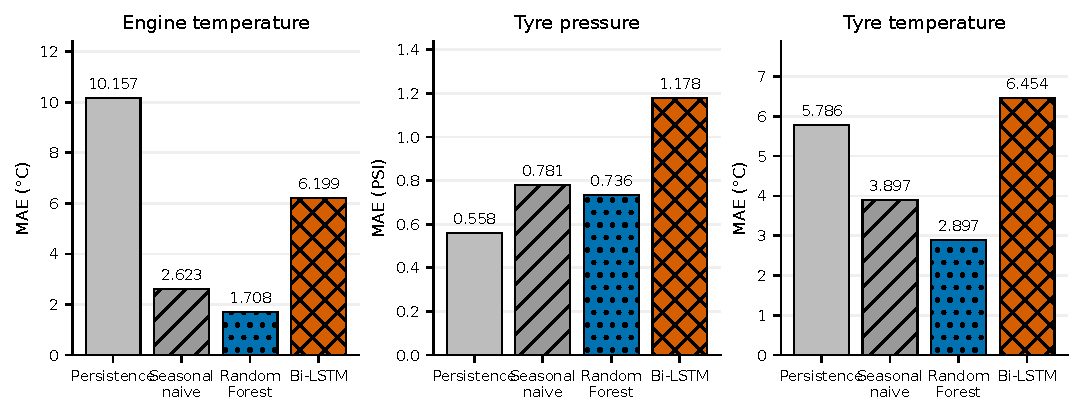
\includegraphics[width=\textwidth]{model_mae_comparison.pdf}
\caption{Mean absolute error from the committed corrected results. Each panel has its own physical-unit axis. Hatching distinguishes models in grayscale.}
\label{fig:mae}
\end{figure*}

For tyre pressure, persistence is strongest, with MAE 0.558 PSI and RMSE 0.979 PSI. Random Forest improves over seasonal naive in MAE but does not improve over persistence. Bi-LSTM has MAE 1.178 PSI, the largest of the four. The result shows why even a nonlinear autoregressive model needs comparison with a latest-value reference.

For tyre temperature, Random Forest again leads, with MAE 2.897\degC\ and RMSE 3.680\degC. Seasonal naive follows at 3.897\degC\ MAE. Bi-LSTM has MAE 6.454\degC\ and negative $R^2$, and also performs worse than persistence. Across the three targets, Bi-LSTM beats the best baseline in zero cases. These are descriptive differences for this experiment; dependent forecasts and a single run do not support a statistical-significance claim.

\subsection{Representative Forecast and Horizon Errors}
Fig.~\ref{fig:forecast} compares actual, Random Forest, and Bi-LSTM engine temperatures for one 24-hour test window. Selection is deterministic: compute Random Forest MAE for every test window, take the median, and select the earliest window whose MAE is closest to that median. The selected zero-based test index is 1464, with first target at December 19, 2024, 00:00. Its Random Forest MAE is 1.579\degC. This is representative only by that explicit criterion; it is not a substitute for the complete test table.

\begin{figure}[t]
\centering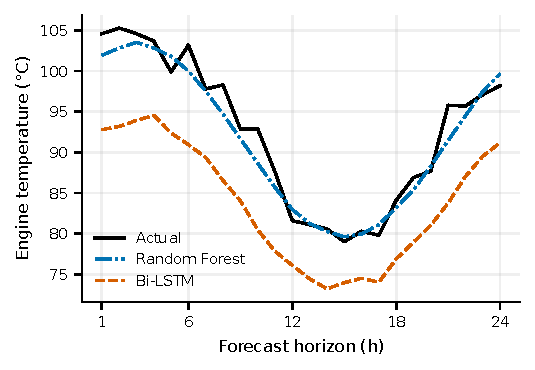
\includegraphics[width=\columnwidth]{engine_24h_forecast_comparison.pdf}
\caption{Deterministically selected 24-hour engine forecast. Forecast issued at 2024-12-18 23:00:00 (dataset clock); selected RF window MAE 1.579 $^\circ$C.
}
\label{fig:forecast}
\end{figure}

Fig.~\ref{fig:horizon} resolves error by elapsed forecast time using aligned predictions. The engine has 24 hourly outputs, whereas each tyre target has eight outputs at three-hour intervals. The plotted values are computed from prediction errors at each horizon, not approximated from aggregate MAE. Persistence is included to put the learned methods in context. The differing curve shapes reinforce that a pooled score does not describe every lead time equally; no monotonic increase of error is assumed.

\begin{figure*}[t]
\centering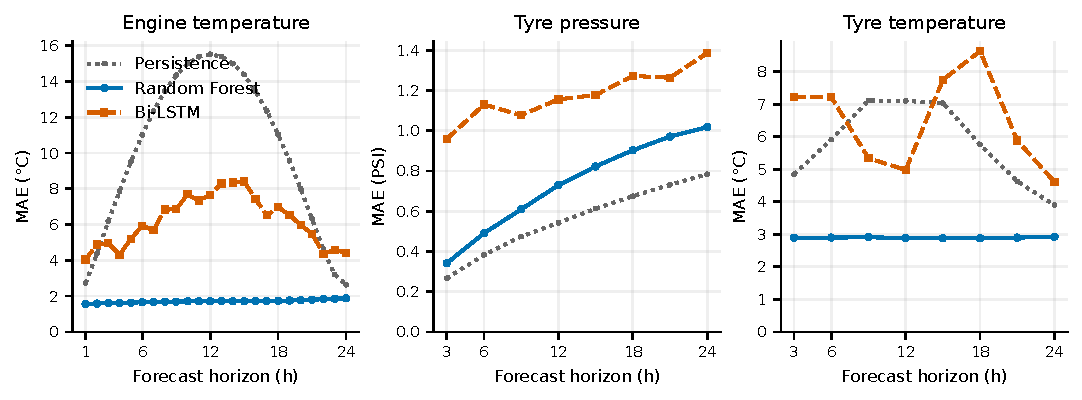
\includegraphics[width=\textwidth]{horizon_mae_comparison.pdf}
\caption{Horizon-wise MAE for persistence, Random Forest, and Bi-LSTM. Engine horizons are 1--24 hours; tyre horizons are 3, 6, \ldots, 24 hours. Each target uses its own physical-unit axis.}
\label{fig:horizon}
\end{figure*}

\subsection{Implications for Model Selection}
Synthetic structure may favor simpler autoregressive or seasonal predictors, while the fixed network and limited training budget may not match each series well. These are possible explanations, not causal findings from an ablation study. The tyre-pressure epoch cap is a concrete reason not to interpret the ranking as proof that Bi-LSTM can never improve. Equally, its capacity does not justify selecting it without evidence.

For this benchmark, Random Forest is the empirical choice for the two temperature targets and persistence for pressure when MAE is the selection criterion. This retrospective ranking does not establish a production selection policy or an unbiased estimate of a newly tuned system. Deployment should evaluate model choices under a pre-declared validation procedure and verify cadence, sensor calibration, threshold meaning, and live data quality. The integrated prototype remains useful as a place to connect a suitable forecast model to a service process, irrespective of model family.

\section{Robustness and Ablation Studies}
Table~\ref{tab:robustness} and Fig.~\ref{fig:robustness} report all five
predeclared Bi-LSTM initialization seeds rather than selecting a favorable
seed. Mean $R^2$ is negative for tyre temperature ($-0.835\pm0.536$), so the
five-seed results do not support a blanket claim of Bi-LSTM superiority.

\begin{table*}[t]
\caption{Five-seed AutoSense Bi-LSTM results. Values are mean $\pm$ sample
standard deviation over seeds 11, 21, 42, 84, and 168.}
\label{tab:robustness}
\centering\small
\begin{tabular}{lrrrr}
\toprule
Dataset & MAE & RMSE & $R^2$ & Unit \\
\midrule
Engine temperature & 5.182 $\pm$ 0.665 & 6.343 $\pm$ 0.655 & 0.531 $\pm$ 0.099 & \degC \\
Tyre pressure & 1.256 $\pm$ 0.221 & 1.532 $\pm$ 0.260 & 0.510 $\pm$ 0.164 & PSI \\
Tyre temperature & 5.731 $\pm$ 0.889 & 7.030 $\pm$ 1.082 & -0.835 $\pm$ 0.536 & \degC \\
\bottomrule
\end{tabular}

\end{table*}

\begin{figure*}[t]
\centering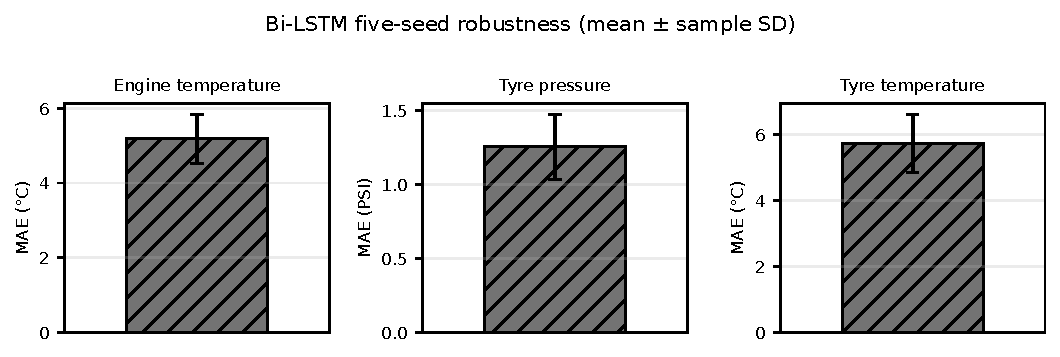
\includegraphics[width=\textwidth]{ieee_upgrade/multiseed_robustness.pdf}
\caption{Five-seed Bi-LSTM MAE. Each panel retains its native physical unit.}
\label{fig:robustness}
\end{figure*}

The seed-42 architecture ablation finds lower Bi-LSTM MAE for engine
temperature (6.199 versus 9.539\degC) and tyre pressure (1.182 versus 1.298
PSI), but lower LSTM MAE for tyre temperature (4.402 versus 6.366\degC).
Table~\ref{tab:architecture} is therefore a controlled first-pass comparison,
not a seed-robust architecture ranking. The causal feature ablation is shown
in Table~\ref{tab:features}. F2 lowers engine-temperature MAE for both RF and
LSTM relative to F0, whereas feature effects differ by target; no feature set
was chosen from test results.

\begin{table*}[t]
\caption{Architecture ablation at seed 42; common chronological splits,
train-only scaling, training budget, and model definitions are retained.}
\label{tab:architecture}
\centering\small
\begin{tabular}{lrrrrr}
\toprule
Dataset & LSTM MAE & Bi-LSTM MAE & LSTM $R^2$ & Bi-LSTM $R^2$ & Unit \\
\midrule
Engine temperature & 9.539 & 6.199 & -0.604 & 0.374 & \degC \\
Tyre pressure & 1.298 & 1.182 & 0.506 & 0.577 & PSI \\
Tyre temperature & 4.402 & 6.366 & -0.034 & -1.194 & \degC \\
\bottomrule
\end{tabular}

\end{table*}

\begin{table*}[t]
\caption{Causal feature-ablation MAE at seed 42. F0: target history; F1:
target plus deterministic calendar; F2: F1 plus causal lag/rolling features.}
\label{tab:features}
\centering\small
\begin{tabular}{llrrrr}
\toprule
Dataset & Model & F0 MAE & F1 MAE & F2 MAE & Unit \\
\midrule
Engine temperature & RF & 1.709 & 1.710 & 1.673 & \degC \\
Engine temperature & LSTM & 9.539 & 7.127 & 5.142 & \degC \\
Tyre pressure & RF & 0.736 & 0.803 & 0.836 & PSI \\
Tyre pressure & LSTM & 1.212 & 2.401 & 2.279 & PSI \\
Tyre temperature & RF & 2.897 & 5.040 & 2.757 & \degC \\
Tyre temperature & LSTM & 4.394 & 4.531 & 4.598 & \degC \\
\bottomrule
\end{tabular}

\end{table*}

\begin{figure*}[t]
\centering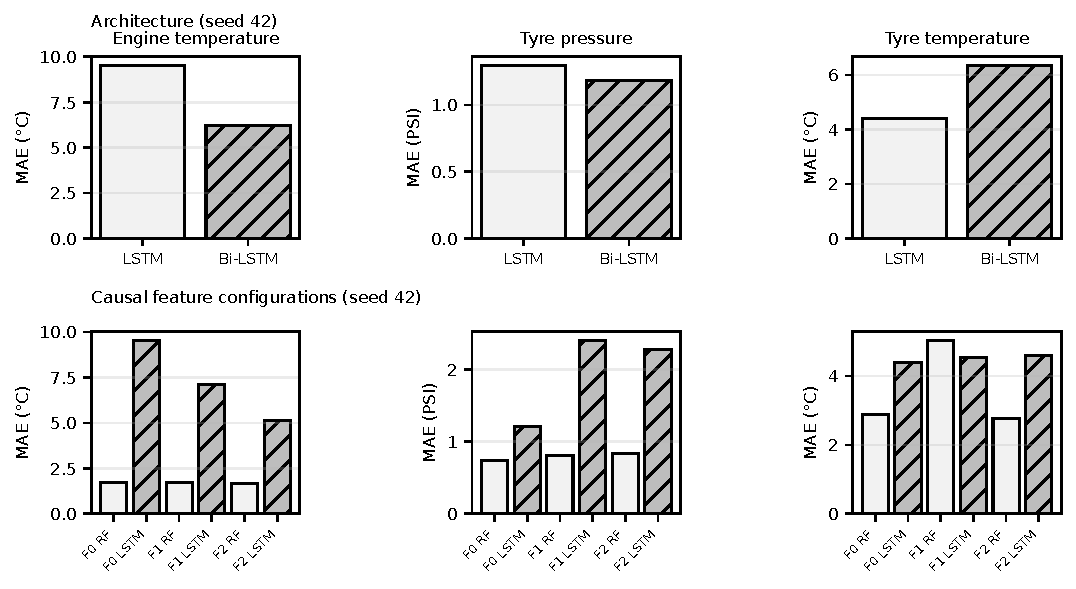
\includegraphics[width=\textwidth]{ieee_upgrade/architecture_feature_ablation.pdf}
\caption{Architecture and causal-feature ablations. Panels use separate
native-unit axes; RF denotes Random Forest.}
\label{fig:ablations}
\end{figure*}

\section{Threshold-Event Evaluation and Uncertainty}
Thresholds are derived from the AutoSense training region only. Table
\ref{tab:events} reports proxy-event scores, including the high tyre-temperature
Bi-LSTM F1 (0.802) together with its false-positive rate of 1.0 and specificity
of 0.0. It is consequently not a useful discriminative alert detector. These
scores concern forecast excursions from data-derived proxy bounds, not
component failures or certified engineering thresholds.

\begin{table*}[t]
\caption{Training-derived proxy threshold-event metrics. FPR is false-positive
rate; these labels are not failure labels.}
\label{tab:events}
\centering\scriptsize
\begin{tabular}{llrrrr}
\toprule
Dataset & Model & Precision & Recall & F1 & FPR \\
\midrule
Engine temperature & Persistence & 0.429 & 0.016 & 0.031 & 0.003 \\
Engine temperature & Seasonal naive & 0.400 & 0.348 & 0.372 & 0.062 \\
Engine temperature & Random Forest & 0.000 & 0.000 & 0.000 & 0.000 \\
Engine temperature & Bi-LSTM & 0.000 & 0.000 & 0.000 & 0.000 \\
Tyre pressure & Persistence & 0.974 & 0.801 & 0.879 & 0.020 \\
Tyre pressure & Seasonal naive & 0.881 & 0.906 & 0.893 & 0.113 \\
Tyre pressure & Random Forest & 0.994 & 0.588 & 0.739 & 0.003 \\
Tyre pressure & Bi-LSTM & 0.000 & 0.000 & 0.000 & 0.000 \\
Tyre temperature & Persistence & 0.800 & 0.176 & 0.288 & 0.089 \\
Tyre temperature & Seasonal naive & 0.763 & 0.775 & 0.769 & 0.487 \\
Tyre temperature & Random Forest & 0.000 & 0.000 & 0.000 & 0.000 \\
Tyre temperature & Bi-LSTM & 0.670 & 1.000 & 0.802 & 1.000 \\
\bottomrule
\end{tabular}

\end{table*}

\begin{figure*}[t]
\centering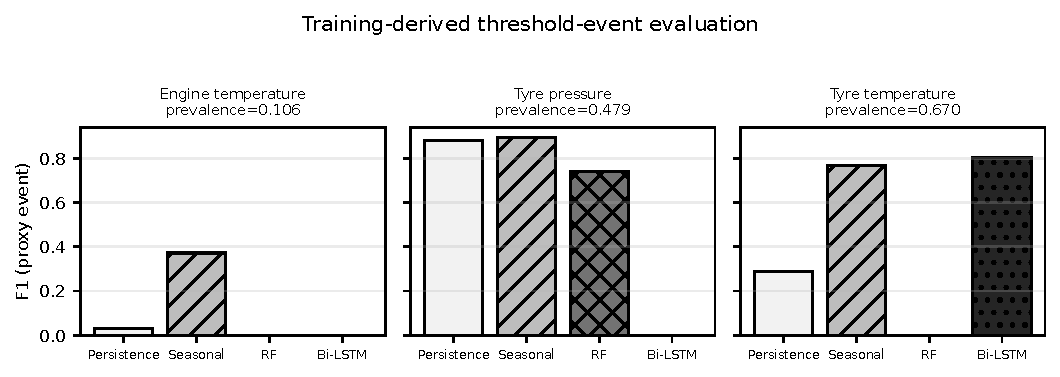
\includegraphics[width=\textwidth]{ieee_upgrade/threshold_event_evaluation.pdf}
\caption{Proxy-event F1 with the event prevalence shown per target.}
\label{fig:events}
\end{figure*}

For the predeclared lowest-MAE corrected baseline against Bi-LSTM, the
2,000-replication non-circular moving-block bootstrap intervals for
MAE(baseline) $-$ MAE(Bi-LSTM) are $[-5.033,-3.955]$\degC for engine
temperature (RF), $[-0.845,-0.356]$ PSI for tyre pressure (persistence), and
$[-3.732,-3.392]$\degC for tyre temperature (RF). Every interval excludes
zero, but dependence-aware intervals are not i.i.d. significance tests or
evidence of operational benefit.

\section{External Benchmark Evaluation on NASA C-MAPSS FD001}
NASA C-MAPSS FD001 is an external \emph{simulated} engine-degradation
benchmark, not real measured flight telemetry. We forecast sensors 9, 11, 14,
and 12 at horizons one through ten cycles, using the fixed disjoint 70/15/15
engine split. C0 uses target history only; C1 uses multivariate history. No
engine occurs in more than one split, sensor selection uses training engines
only, and the scaler is fitted on training engines only.

Table~\ref{tab:cmapss} gives training-range-normalized macro results, which
avoid averaging incomparable native sensor units. In C1, Random Forest achieves
the lowest macro normalized MAE (0.03406), lowest normalized RMSE (0.04278),
and highest $R^2$ (0.88907) among the evaluated seed-42 model configurations.
These values describe fixed configurations rather than a tuned model contest.
The results were recorded with TensorFlow 2.20.0 and scikit-learn 1.6.1,
unlike the 2.18.0/1.9.0 AutoSense runs.

\begin{table*}[t]
\caption{C-MAPSS FD001 macro-average training-range-normalized metrics.
Bi-LSTM uses the three predeclared seeds; C0 is target-only and C1 is
multivariate history.}
\label{tab:cmapss}
\centering\small
\begin{tabular}{llrrrr}
\toprule
Configuration & Model & Seed & NMAE & NRMSE & $R^2$ \\
\midrule
C0 & Bi-LSTM & 11 & 0.03543 & 0.04442 & 0.87980 \\
C0 & Bi-LSTM & 42 & 0.03574 & 0.04481 & 0.87820 \\
C0 & Bi-LSTM & 84 & 0.03654 & 0.04582 & 0.87163 \\
C0 & LSTM & 42 & 0.03582 & 0.04490 & 0.87747 \\
C0 & Persistence & 42 & 0.04722 & 0.05988 & 0.78467 \\
C0 & Random Forest & 42 & 0.03472 & 0.04362 & 0.88438 \\
C1 & Bi-LSTM & 11 & 0.03499 & 0.04387 & 0.88457 \\
C1 & Bi-LSTM & 42 & 0.03483 & 0.04366 & 0.88536 \\
C1 & Bi-LSTM & 84 & 0.03505 & 0.04393 & 0.88414 \\
C1 & LSTM & 42 & 0.03460 & 0.04341 & 0.88620 \\
C1 & Random Forest & 42 & 0.03406 & 0.04278 & 0.88907 \\
\bottomrule
\end{tabular}

\end{table*}

The fixed early ($<0.5$), mid ($0.5$ to $<0.8$), and late ($\geq0.8$)
normalized-life bins are used only to stratify held-out sensor-forecasting
error after prediction; they do not create an RUL target. Fig.~\ref{fig:cmapss}
summarizes the C1 sensor, horizon, and stage views. The stage script itself
records TensorFlow 2.18.0/scikit-learn 1.9.0, but its inputs are the accepted
forecast artifacts recorded under TensorFlow 2.20.0/scikit-learn 1.6.1; that
inherited environment deviation remains part of the provenance.

\begin{figure*}[!t]
\centering
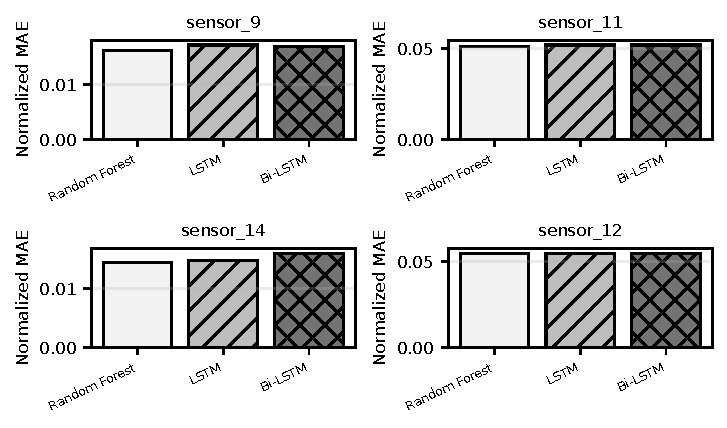
\includegraphics[width=.70\textwidth]{ieee_upgrade/cmapss_external_validation.pdf}\par
\smallskip
\begin{minipage}[t]{.37\textwidth}
\centering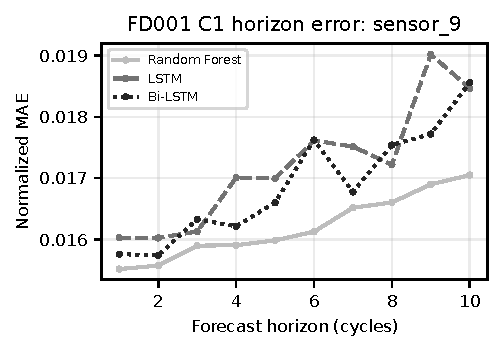
\includegraphics[width=\linewidth]{ieee_upgrade/cmapss_horizon_mae.pdf}
\end{minipage}\hfill
\begin{minipage}[t]{.59\textwidth}
\centering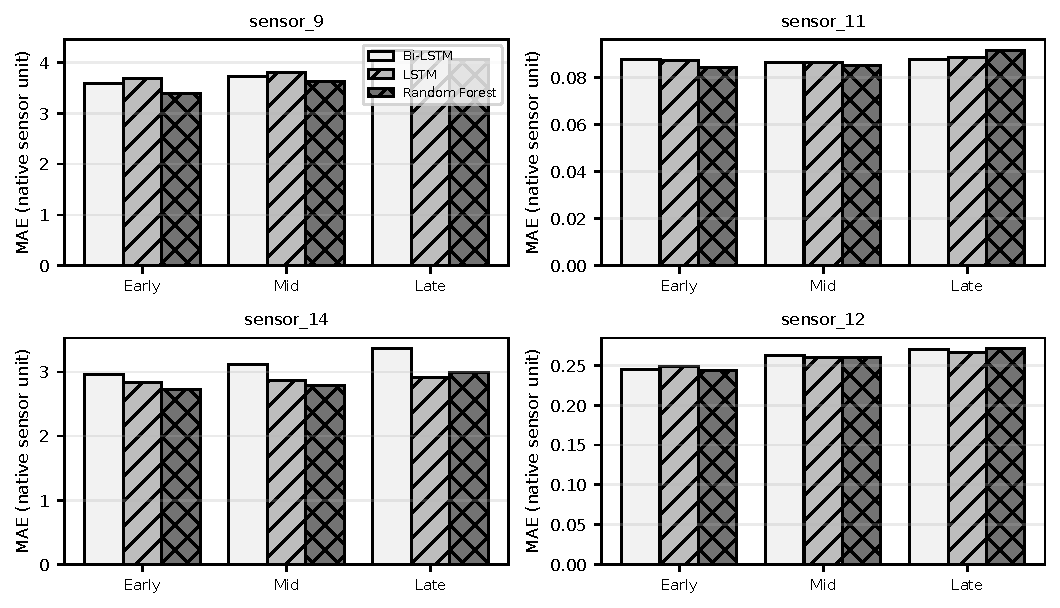
\includegraphics[width=\linewidth]{ieee_upgrade/cmapss_stage_error.pdf}
\end{minipage}
\caption{C-MAPSS FD001 C1 results: top, normalized MAE by target sensor; the
displayed Bi-LSTM bar is seed 42, while all three predeclared seeds remain in
Table~\ref{tab:cmapss}. Bottom left, normalized MAE by forecast horizon for
sensor 9 (Bi-LSTM seed 42). Bottom right, MAE stratified by fixed
normalized-life stage; panels use native units and display Bi-LSTM seed 42 for
readability.}
\label{fig:cmapss}
\end{figure*}
\FloatBarrier

\section{Prototype Integration and Workflow Validation}
The repository provides three complementary forms of integration evidence. First, firmware implements sensor parsing, telemetry payloads, and platform transmission. Second, platform scripts and interface captures demonstrate the intended ingestion and forecast-display interfaces. Third, Salesforce Apex implements alert import and vehicle-status callbacks. These artifacts support technical feasibility at the prototype level; the present work inspects them without contacting live endpoints or rerunning hardware and Salesforce tests.

Fig.~\ref{fig:interfaces} retains the original fleet-map, sensor-view, and
Salesforce Vehicle Alert screenshots. They establish the existence and layout
of monitoring interfaces. Displayed vehicle names, readings, and thresholds
are demonstration context, not the held-out synthetic benchmark or a validated
operating fleet. The forecast-display screenshot is omitted to avoid confusing
legacy forecast curves with the corrected comparison.

The alert-ingestion service maps identifiers, severity, description, and status
to a custom Vehicle Alert record. The separate Salesforce panel in
Fig.~\ref{fig:interfaces} shows that record type; it is not a screenshot of a
Salesforce Case. A separate trigger detects changes to a vehicle's status and
calls the status service. This demonstrates the implemented feedback mechanism
in source code, but not that closing a Case caused that update in a reproducible
test.

\begin{figure*}[!t]
\centering
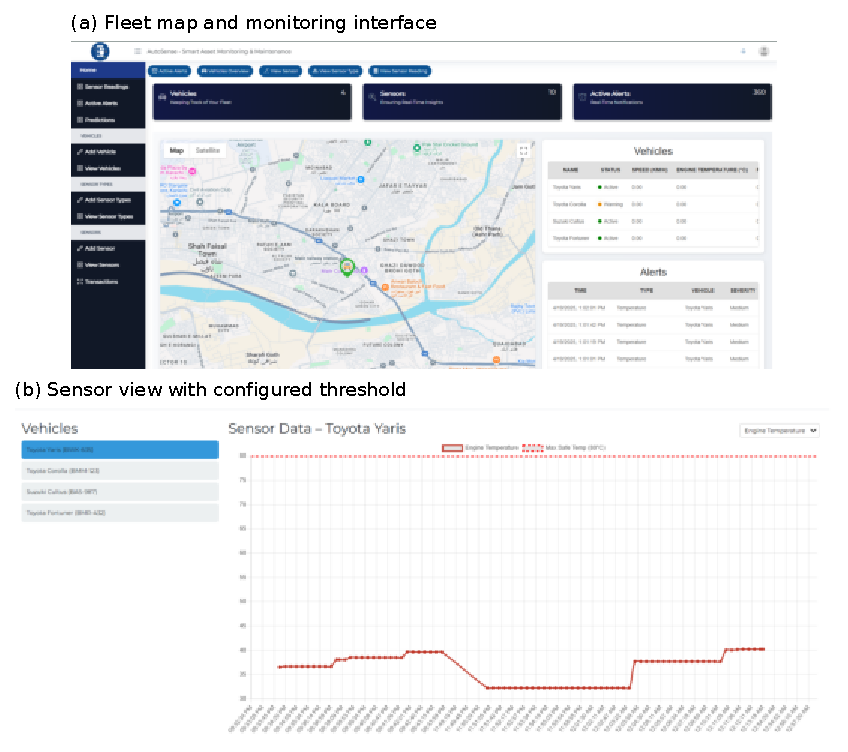
\includegraphics[width=.70\textwidth]{prototype_interfaces.pdf}\par
\smallskip
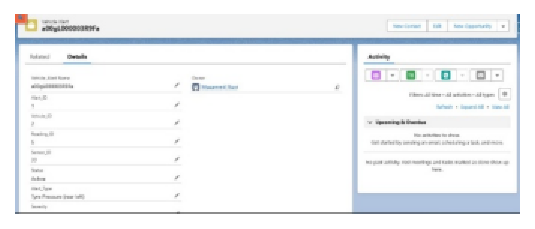
\includegraphics[width=.34\textwidth]{salesforce_alert.pdf}
\caption{Retained prototype interface evidence from the original project:
(a) fleet map and monitoring, (b) sensor view with a configured threshold, and
(c) a Salesforce Vehicle Alert record. The screenshots are interface
demonstrations, not scientific test observations, verified Case creation, or
verified Flow automation. The source raster for (c) is low resolution.}
\label{fig:interfaces}
\end{figure*}
\FloatBarrier

Case creation and assignment through Flow, the resolution-to-vehicle linkage, and live forecast-endpoint operation are described in the original project but lack sufficient exported configuration or execution traces for independent reproduction. No latency distribution, success-rate denominator, environmental-test record, or measured downtime/cost study was found in the reviewed evidence. Consequently, the paper makes no numerical integration-reliability or response-time claim. A future integration test should trace a timestamped sensor event through alert creation, Case assignment, closure, and dashboard feedback with recorded outcomes.

\section{Limitations}
The principal limitation is synthetic data: the results measure forecasting on generator-produced signals rather than external real-fleet observations. The hardware and software artifacts do not establish domain transfer, automotive robustness, or aviation operational validation. Sensor placement and calibration also determine whether a displayed temperature is a useful proxy for engine condition.

The corrected benchmark's main comparison uses one chronological holdout and a
fixed limited training budget with no full hyperparameter search. Five-seed
variation is reported only for the AutoSense Bi-LSTM, and the LSTM/Bi-LSTM
architecture comparison remains a seed-42 first pass. Overlapping forecast
origins yield dependent errors; the moving-block intervals address this
dependence for the predeclared baseline-versus-Bi-LSTM MAE comparisons but do
not convert the study into repeated-split validation. Negative $R^2$ and
physical-unit errors are retained rather than replaced by normalized metrics.

The C-MAPSS study is an external simulated benchmark rather than a real fleet
or measured flight-telemetry validation. It uses a different recorded
TensorFlow/scikit-learn environment from some AutoSense phases; version
heterogeneity limits exact cross-environment reproducibility even though the
pre-registered sources, splits, sensors, scalers, settings, hashes, and
prediction-engine IDs were validated. Feature-ablation conclusions likewise
belong to their recorded TensorFlow 2.20.0/scikit-learn 1.6.1 environment.

There are no maintenance-outcome labels, direct failure or remaining-useful-life targets, or measured downtime and cost reductions. Forecast accuracy alone cannot establish operational maintenance benefit or calibrated alarm risk. Case/Flow configuration and live transaction logs are incomplete in the repository, so the fully closed service loop remains less strongly evidenced than its constituent ingestion and status components. The legacy integration scripts have not been migrated to the corrected benchmark protocol.

\section{Conclusion and Future Work}
This work presents an integrated IoT-to-enterprise prototype and a corrected
comparative study of 24-hour multi-step sensor forecasting. The available
firmware, platform interfaces, and Salesforce code support prototype-level
technical feasibility, with explicit limits on workflow validation. On three
synthetic datasets, Random Forest provides the lowest temperature MAEs and
persistence the lowest pressure MAE. Five-seed robustness, fixed architecture
and causal-feature ablations, proxy threshold-event metrics, and moving-block
intervals reinforce the need for evidence-based model selection. A separate,
engine-disjoint C-MAPSS FD001 simulated-benchmark study extends the analysis to
multivariate sensor forecasting, while retaining its environment deviation.

Future work should prioritize real fleet data collection, genuine failure and maintenance labels, and external validation. Uncertainty-aware forecasts and richer CAN bus features should be assessed under a pre-declared model-selection protocol with strong baselines. More complex architectures, including Transformers, would require that same evidential standard. Completing and exporting Case/Flow configuration, validating the live feedback loop, and measuring maintenance outcomes would connect forecast quality to practical service value.

\bibliographystyle{IEEEtran}
\bibliography{references}
\end{document}
